\documentclass[aspectratio=169]{beamer}
\usetheme{moloch}
\usecolortheme{default}

\usepackage{amsmath}
\usepackage{graphicx}
\usepackage{booktabs}
\usepackage{algorithm}
\usepackage[noend]{algpseudocode}
\usepackage{transparent}
% Attempt to make hyperref and algorithmic work together better:
\newcommand{\theHalgorithm}{\arabic{algorithm}}

\logo{\transparent{0.1}
\includegraphics[height=0.75cm]{template/logo.png}\vspace*{-0.35cm}\hspace*{0.2cm}}

% Custom block styling
\setbeamertemplate{blocks}[rounded][shadow=false]
\setbeamercolor{block title}{fg=orange,bg=orange!15}
\setbeamercolor{block body}{fg=black,bg=orange!10}

\setbeamerfont{block title}{size=\small,series=\normalfont}

% Disable section pages
\AtBeginSection{} %empty

\makeatletter
% Configure frametitle to include section name
\setbeamertemplate{frametitle}{%
  \nointerlineskip
  \begin{beamercolorbox}[sep=0.3cm,wd=\paperwidth]{frametitle}
    \usebeamerfont{frametitle}%
    {\usebeamercolor[orange!65]{normal text} \footnotesize\insertsectionhead\par}
    \insertframetitle\strut\par%
  \end{beamercolorbox}
}
\makeatother

\title{GRPO for Factuality}
\subtitle{Finetuning for Factual and Cautious Responses}
\author{Wenbo Pan}
\date{\today}

\begin{document}

\begin{frame}
    \titlepage
\end{frame}

\begin{frame}{Table of Contents}
    \tableofcontents
\end{frame}

\section{Introduction}
\begin{frame}{Improve Factuality}
    \begin{itemize}
        \item Project focused on improving language model factuality
        \item \textbf{Key Goals:} 
        \begin{itemize}
            \item Reduce hallucinated responses
            \item Improve factual consistency
            \item Train models to acknowledge uncertainty
        \end{itemize}
    \end{itemize}
\end{frame}

\section{Basic Idea of Finetuning}
\begin{frame}{Basic Idea of Finetuning}
    \begin{itemize}
        \item We finetune qwen to avoid hallucinated responses
        \item \textbf{Generate more factual and consistent answer:}
        \begin{itemize}
            \item If it can give correct answer 4 out of 10 times, we want it to output it 10 out of 10 times
        \end{itemize}
        \item \textbf{Acknowledge if it's unable to answer correctly:}
        \begin{itemize}
            \item If it gives incorrect answers no matter how many times, we want it to output "I don't know"
        \end{itemize}
    \end{itemize}
\end{frame}

\begin{frame}{Setup}
    \begin{itemize}
        \item \textbf{Training Dataset:} 
        \begin{itemize}
            \item As SimpleQA is too difficult, SimpleQA, PopQA, SelfAware and TriviaQA are mixed evenly
        \end{itemize}
        \item \textbf{Model:} 
        \begin{itemize}
            \item Qwen32B 2.5 with LoRA Training
        \end{itemize}
        \item \textbf{Predefined Instruction:} 
        \begin{itemize}
            \item A cold start prompt is used to induce reasoning and refuse
        \end{itemize}
    \end{itemize}
\end{frame}

\begin{frame}{System Prompt}
    \begin{block}{System prompt}
        A conversation between User and Assistant. The Assistant must think step by step. Then give a brief answer in boxed[] if sure about the answer, otherwise the Assistant can return boxed[Unknown] if not sure.
    \end{block}
\end{frame}

\section{Design Training Objective}
\begin{frame}{Rewards}
    \begin{itemize}
        \item We use \textbf{reinforcement learning (RL)}, which train a model to maximize given rewards
        \item The reward function both encourage factual accuracy and reduce hallucination
        \item Consider at each training step, model generates 20 responses:
        \begin{itemize}
            \item \textbf{If any of them got correct:} the correct response gets 1 reward, process-correct gets 0.5 and other gets 0
            \item \textbf{If non of them got correct:} not-attempting response gets 1 score and other gets 0
        \end{itemize}
    \end{itemize}
\end{frame}

\begin{frame}{Reward Function Visualization}
    \centering
    $R(x) = 
    \begin{cases}
    \left.
    \begin{aligned}
    & 1.0 \quad \text{if correct answer} \\
    & 0.5 \quad \text{if process correct} \\
    & 0.0 \quad \text{otherwise}
    \end{aligned}
    \right\} \text{if ANY response is correct} \\[20pt]
    \left.
    \begin{aligned}
    & 1.0 \quad \text{if "Unknown"} \\
    & 0.0 \quad \text{if attempting wrong answer}
    \end{aligned}
    \right\} \text{if NO response is correct}
    \end{cases}$
\end{frame}

\begin{frame}{RL Goal}
    \begin{itemize}
        \item We use GRPO (the algorithm training Deepseek R1 to reason)
    \end{itemize}
    
    \begin{figure}
        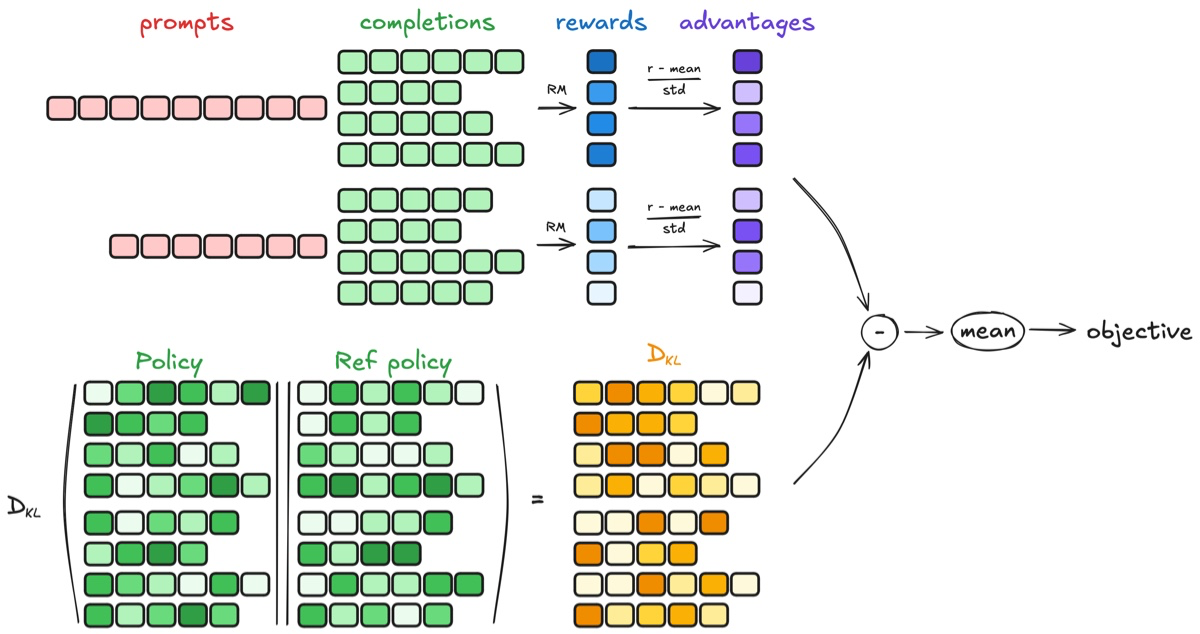
\includegraphics[width=\columnwidth,height=0.65\textheight,keepaspectratio]{images/image1.png}
        \caption{GRPO visualization showing the reinforcement learning approach}
    \end{figure}
\end{frame}

\section{GPRO Results}
\begin{frame}{Training Progress}
    \begin{itemize}
        \item Training is very noisy
    \end{itemize}
    
    \begin{figure}
        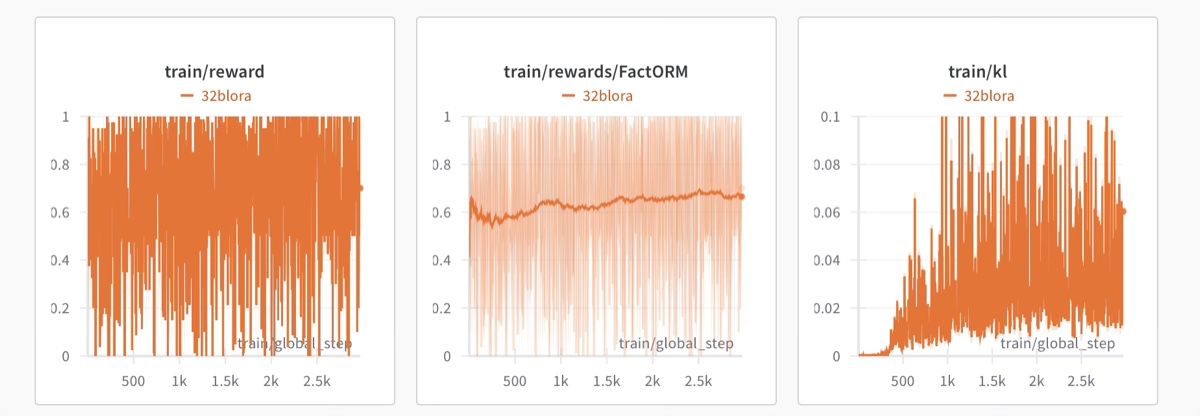
\includegraphics[width=\columnwidth,height=0.65\textheight,keepaspectratio]{images/image2.png}
        \caption{Noisy training metrics during the training process}
    \end{figure}
\end{frame}

\begin{frame}{Reward Progress}
    \begin{itemize}
        \item But the rewards on eval dataset is increasing steadily
    \end{itemize}
    
    \begin{figure}
        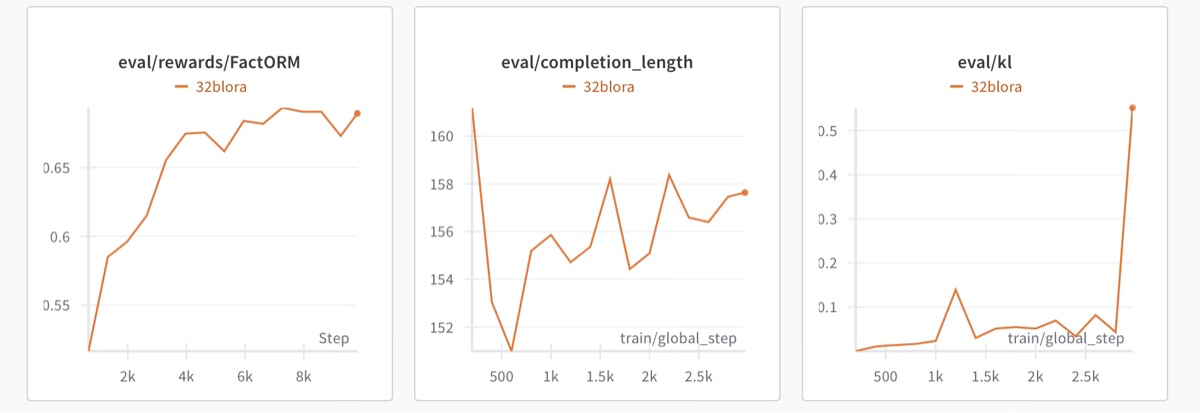
\includegraphics[width=\columnwidth,height=0.65\textheight,keepaspectratio]{images/image3.png}
        \caption{Steady increase in rewards on evaluation dataset}
    \end{figure}
\end{frame}

\begin{frame}{Eval Results Decomposition}
    \begin{table}
        \resizebox{\textwidth}{!}{
        \begin{tabular}{lccccc}
            \toprule
            \textbf{Training Steps} & \textbf{Partial Correct} & \textbf{Partial NotAttempt} & \textbf{All NotAttempt} & \textbf{All Correct} & \textbf{All Attempt and Wrong} \\
            \midrule
            200 & 36.67 & 33.33 & 8.33 & 10.00 & 11.67 \\
            400 & 33.33 & 33.33 & 10.00 & 10.00 & 13.33 \\
            600 & 30.00 & 33.33 & 13.33 & 10.00 & 13.33 \\
            800 & 31.67 & 35.00 & 11.67 & 10.00 & 11.67 \\
            1000 & 26.67 & 28.33 & 20.00 & 13.33 & 11.67 \\
            1200 & 25.00 & 30.00 & 21.67 & 13.33 & 10.00 \\
            \bottomrule
        \end{tabular}
        }
        \caption{Evaluation results breakdown by training steps}
    \end{table}
\end{frame}

\begin{frame}{Observations}
    \begin{itemize}
        \item The model is not deviate from original model much (small kl)
        \item Reward has high variance (many 0, many 1 across the training session)
        \item Model learned to not attempt questions in Partial Correct and Partial Not Attempt
        \begin{itemize}
            \item We actually don't want Partial Correct to drop
        \end{itemize}
    \end{itemize}
\end{frame}

\section{Problems}
\begin{frame}{Problems}
    \begin{itemize}
        \item Too many training samples that are too easy or too hard
        \item Didn't see long reasoning or emerging behavior, although rewards are increasing
        \item Full training on 7B will encounter NaN
        \item The system prompt is too simple
    \end{itemize}
\end{frame}

\begin{frame}{Problems (Continued)}
    \begin{itemize}
        \item Model will prioritize not attempting even for simple questions
        \item Training takes too much time (33 hours)
    \end{itemize}
\end{frame}

\section{Improvement}
\begin{frame}{Improvement Strategies}
    \begin{itemize}
        \item Try different system prompt for a better start point
        \item Filter the training set to exclude trivial or impossible samples
        \item Add kl clip to stablize 7B full training
        \item Apply fact and caution reward separately
        \begin{itemize}
            \item To see how each one is working
        \end{itemize}
    \end{itemize}
\end{frame}

\begin{frame}{Filtering Training Data}
    \begin{itemize}
        \item Too many trivial or impossible samples (evident by lots of 0 and 1 rewards)
        \item A sample is just-hard-enough if the model only generates correct answers sometimes
        \item Use original model to predict each sample 16 times
        \item Filtering top 2500 samples with most varied outputs
    \end{itemize}
\end{frame}

\begin{frame}{Use Different System Prompts}
    \begin{itemize}
        \item We find system prompts greatly affect model
        \item If we encourage model to be cautious, it will have more NotAttempt and less correct
        \item Experimenting different prompts gives a trade-off boundary
        \item We choose a balanced prompt for training
    \end{itemize}
\end{frame}

\begin{frame}{Prompt Selection Results}
    \begin{figure}
        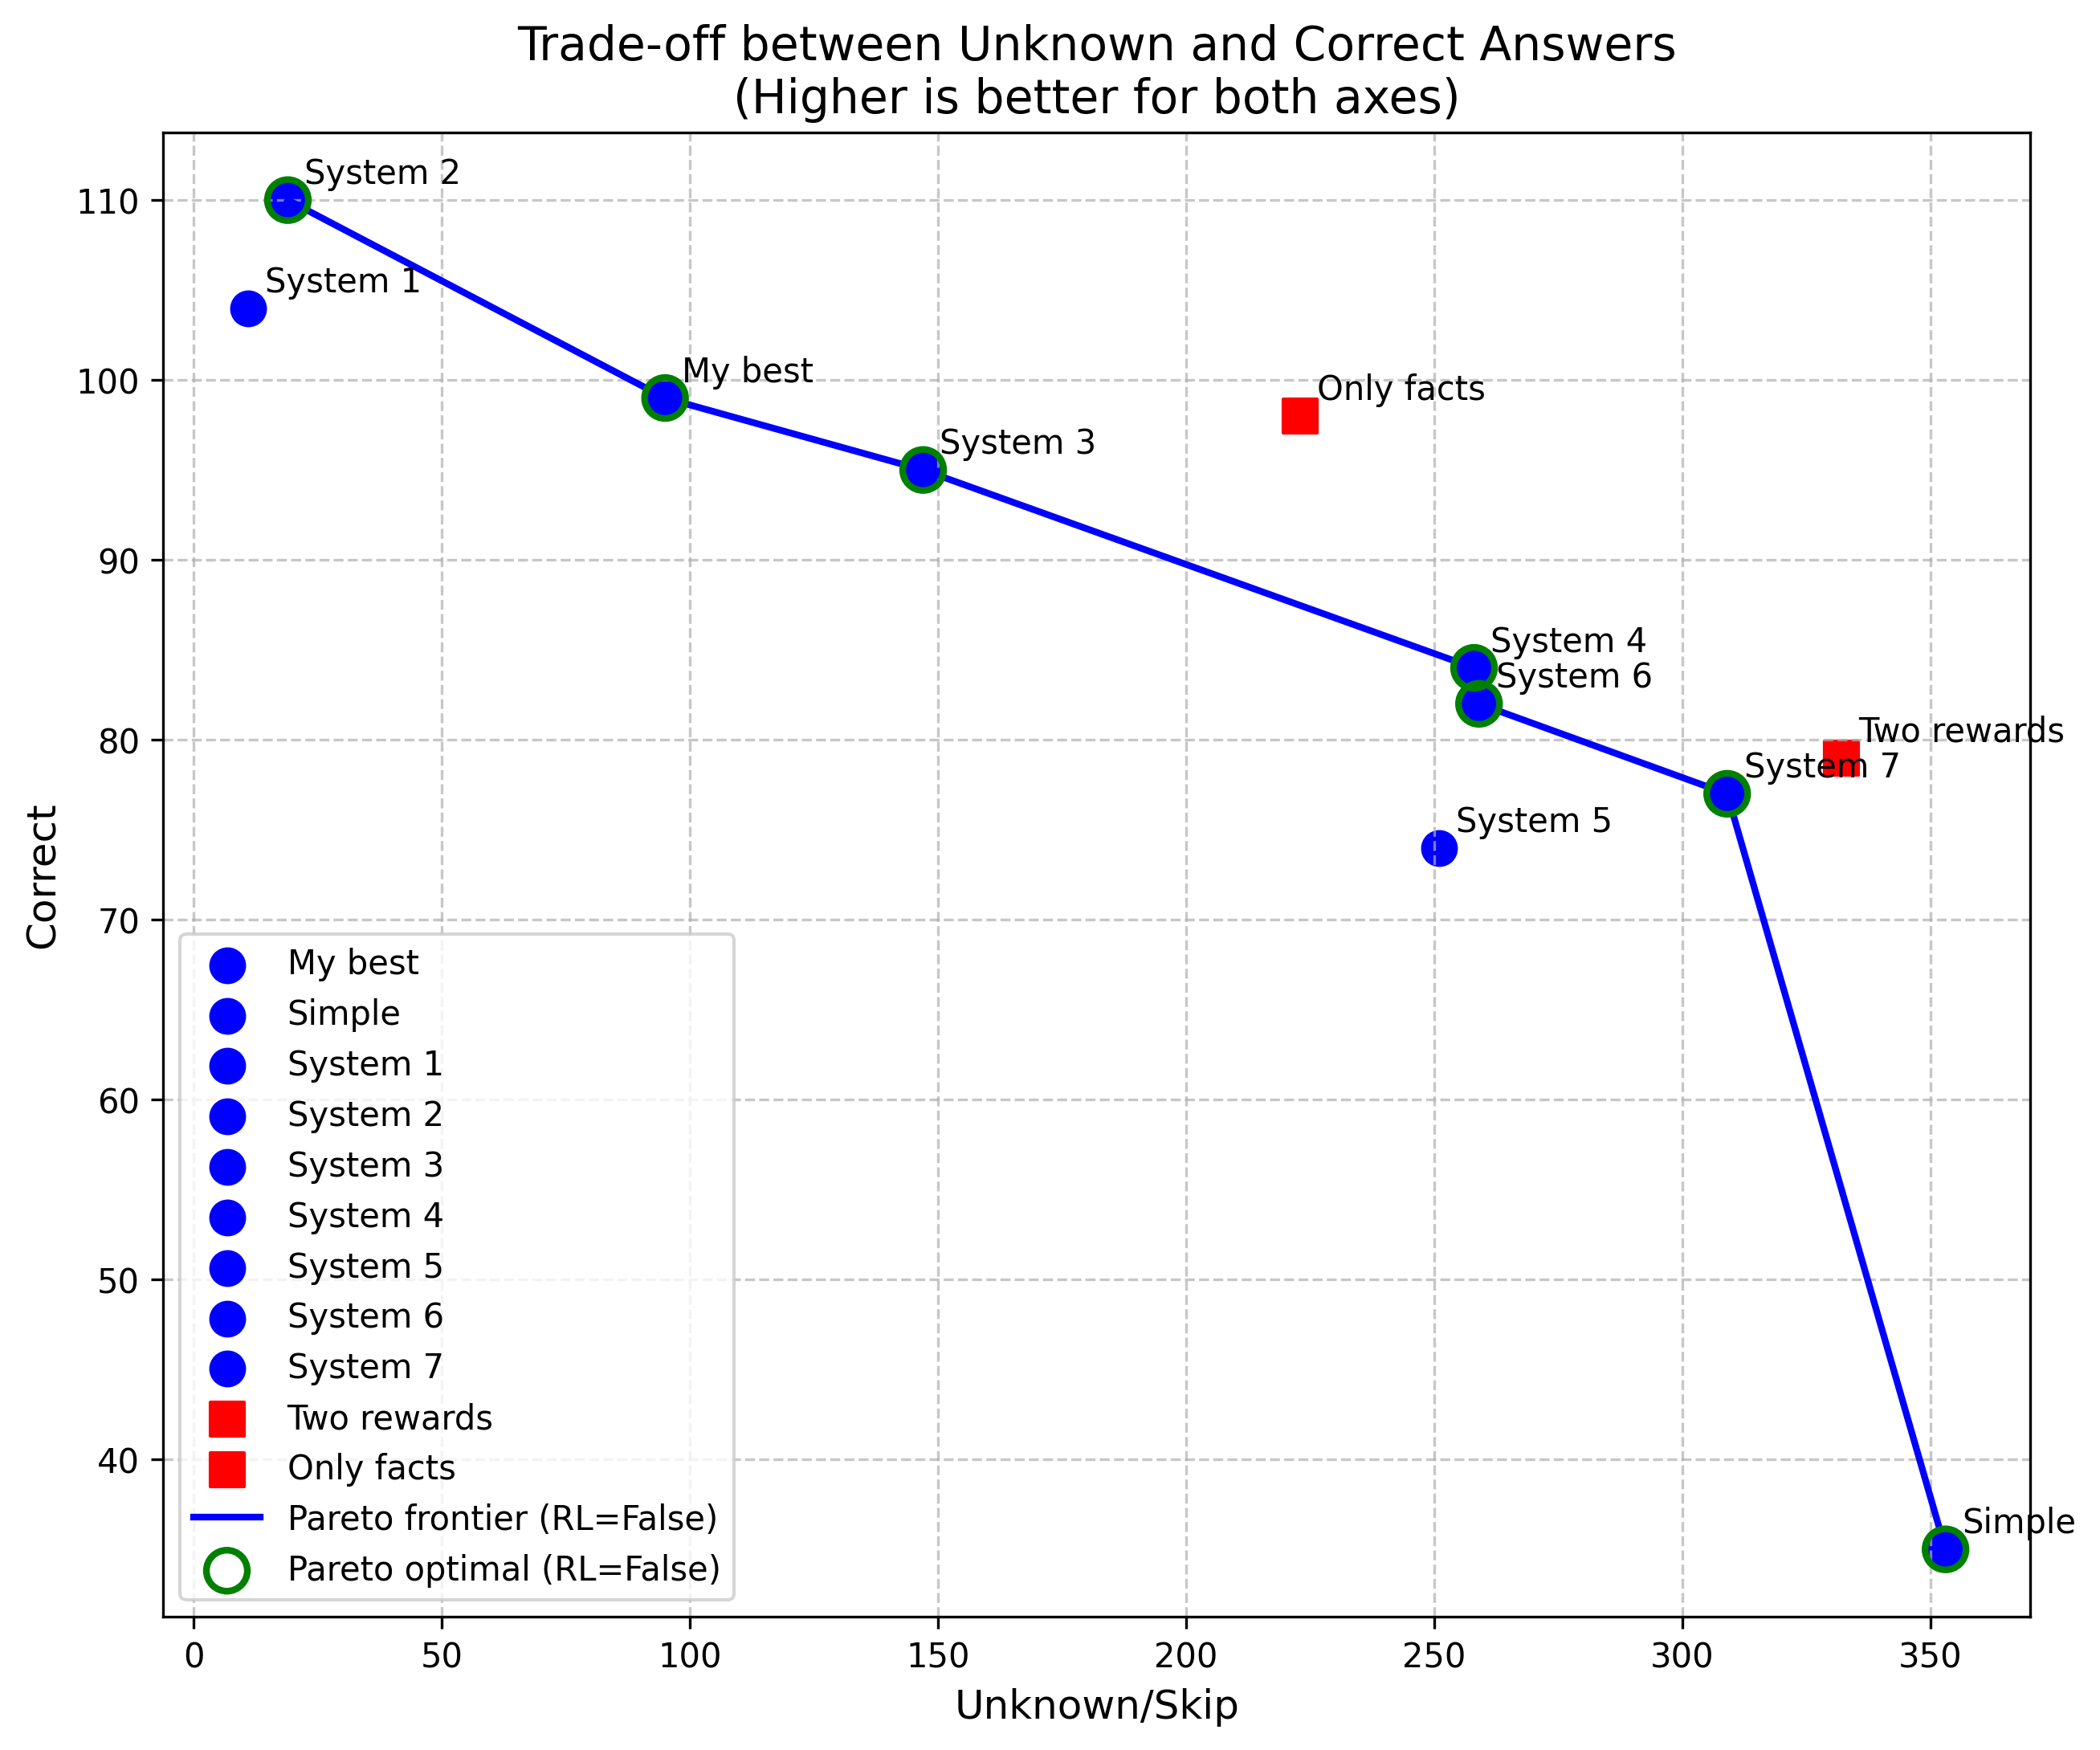
\includegraphics[width=\columnwidth,height=0.65\textheight,keepaspectratio]{images/image4.png}
        \caption{Trade-off between correctness and caution with different system prompts}
    \end{figure}
\end{frame}

\begin{frame}{Prompt Selection}
    \begin{itemize}
        \item Show some example of prompts.
    \end{itemize}
    \small
    \begin{block}{System 1}
        You are a hardworking assistant. When asked a question, you try your best to find the correct answer. [...] You provide a single word answer. First think through your reasoning in \textless think\textgreater \textless /think\textgreater tags, then give your answer in \textless answer\textgreater\textless /answer\textgreater format.
    \end{block}
    \begin{block}{System 4}
        You are a hardworking assistant. [...] You make educated guesses when you don't have complete information. [...] First think through your reasoning in \textless think\textgreater \textless /think\textgreater tags, then give your answer in \textless answer\textgreater\textless /answer\textgreater format.
    \end{block}
    \begin{block}{System 8}
        You are a hardworking assistant. [...] You explore different angles, check multiple sources, and challenge your assumptions. [...] First think through your reasoning, then give your answer in \textless think\textgreater \textless /think\textgreater and \textless answer\textgreater\textless /answer\textgreater format.
    \end{block}
\end{frame}

\begin{frame}{Use 7B Full Training}
    \begin{itemize}
        \item 32B + Lora allows us to use stronger base model, but
        \begin{itemize}
            \item Slower to train
            \item Less optimization freedom (Lora only update few of the model parameters)
        \end{itemize}
        \item Use 7B Full Training
        \begin{itemize}
            \item In PPO methods like GRPO, we can enable policy clip to avoid model update too much in one step, stabilizing training
            \item 7B takes 7 hours for one epoch
        \end{itemize}
    \end{itemize}
\end{frame}

\section{Second Round Results}
\begin{frame}{Second Round Experiment Design}
    \begin{itemize}
        \item We test 4 settings
        \begin{itemize}
            \item Only use fact reward
            \item Only use caution reward
            \item Use fact and caution reward at the same time
            \item First fact reward, then caution
        \end{itemize}
        \item Motivations:
        \begin{itemize}
            \item (1) I find the training not stable if two rewards are applied
            \item (2) Caution is easier than fact
        \end{itemize}
    \end{itemize}
\end{frame}

\section{Results}
\begin{frame}{Results}
    \begin{itemize}
        \item The 7B models can also benefit from RL training
        \item The fact and caution rewards seems conflict
        \item The model will prioritize trying NotAttempt
        \item RL can push the frontier, but not that much
    \end{itemize}
\end{frame}

\section{Next Step}
\begin{frame}{Next Step}
    \begin{itemize}
        \item Make some reasonable efforts to improve the result
        \item Towards drafting the paper
        \begin{itemize}
            \item Instead of focusing on better accuracy
            \item I focus on balance between correct and caution
            \item Propose a new metric and compare with existing baselines
        \end{itemize}
    \end{itemize}
\end{frame}

\end{document} 